\chapter{Theory}
\label{chap:Theory}

\section{Introduction}
This chapter provides an explanation of different types of concepts that is essential to understand before reading the rest of the thesis. It covers various forms of software testing, multiple techniques of security testing, and other relevant information deemed necessary to understand the thesis.

\section{Software Development Life Cycle}
\acrlong{sdlc} can be defined as \textit{"structured process that enables the production of high-quality, low-cost software, in shortest possible production time. The goal of the \acrshort{sdlc} is to produce superior software that meets and exceeds all customer expectations and demands"}\cite{sdlc1}. SDLC consists of several phases providing a software development testing and deployment framework. It is also worth noting that the \acrlong{sdlc} is an iterative process \cite{sdlcinterative}. Each life cycle phase can undergo multiple iterations and be repeated, with each iteration building upon the previous one. This iterative approach facilitates continuous improvement and refinement of the software product, resulting in a final product that meets or exceeds customer needs and expectations. By leveraging this iterative approach, software development teams can ensure that their software is of the highest quality while still being completed within a reasonable time frame and cost. Below are the five phases that fulfill the \acrshort{sdlc}. 

\subsection{Planning} 
Planning is the first phase of the \acrshort{sdlc} \cite{planningphase}. During this phase, the team determines the project's goals and objectives. The team should discuss resources, costs, and time and create a timeline for the work during this phase. Additionally, the team should develop a project plan where they identify, prioritize, and assign tasks and resources necessary to construct the structure. This stage is repeated when changes or new features are presented. In a \acrshort{cicd} pipeline, the team receives feedback and includes it in a new planning phase.

\subsection{Implementation}
In the implementation phase, the actual development of the software takes place \cite{ImplementationSDLC}. The software design is translated into code using programming languages during implementation. Once the team completes and reviews the code, they initiate the build process and conduct several security scans. The implementation phase is considered important since this is the phase that involves the actual development of the software and the preparation of the software for deployment into the environment.  
 
\subsection{Testing}
In the testing phase, the development team verifies that the software fulfils functional, performance, and quality criteria established in earlier stages of the \acrshort{sdlc} \cite{TestingSDLC}. The software is subjected to both manual user testing and automated testing to detect and correct possible defects. In the testing phase, the development team ensures that the software meets the user's requirements.
 
\subsection{Deployment}
In the deployment phase, releasing the software into the environment can be considered the main priority \cite{DeploymentSDLC}. In this phase, the deployment team works with the development team and other stakeholders to plan the release of the software in order to ensure a seamless process. The plan also includes creating the deployment timeline, selecting a method for the deployment, and defining the software's environment. Initially, the deployment process of an application may take a considerable amount of time. However, once the application has been deployed for the first time, subsequent updates can be deployed much faster because the same setup is reused, significantly reducing deployment time. 

\subsection{Maintenance} 
In the maintenance phase, the software is monitored to ensure it functions according to its intended design \cite{MaintenanceSDLC}. The team does any refactoring and upgrades it is if needed. Software monitoring can be done differently depending on how the maintenance phase has been set up. However, the most common way of monitoring is usually through real-time reporting or ad-hoc reporting systems, which are automatically generated within the software created and then sent to the company that created it. 


\begin{figure}[H]
    \centering
    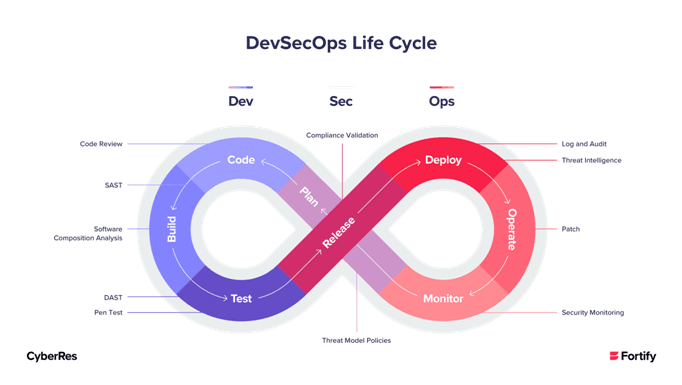
\includegraphics[width=0.8\columnwidth]{Images/devsec.png}
    \caption{DevSecOps Life Cycle}
    \label{fig: DevSecOps Life Cycle}\cite{devsecopsbilde}
\end{figure}


\section{Functional testing vs. security testing}
\label{Functional Testing vs Security Testing}
Software testing is an extensive area, and each test varies according to its purpose or process - but the primary goal of software testing is to verify the quality of software systems through planned and structured testing under controlled conditions \cite{difftesting}. Functional testing emphasizes the software's behavior and that the software is working as expected. The functional test cases are based on the software requirements specified by the stakeholder. Several functional testing methodologies, such as unit and integration testing, can be conducted. 
\\~\\
Unit testing involves testing small code components, known as units, to determine if the units behave as expected\cite{unitvsintergration}. These tests are typically executed early in the \acrshort{sdlc} to identify bugs early on and save time in the rest of the process. The unit testing aims to run tests on all possible components in an isolated test environment to confirm if the code operates as anticipated. On the other hand, integration testing evaluates how the previously tested components perform when integrated into a more extensive system and communicate across various components.
\\~\\
On the other hand, security testing wants to break the software to uncover vulnerabilities and verify its security features \cite{whysectest}. The testing aims to identify all possible weaknesses that attackers might exploit. During the testing, the testers perform the test from the attacker's point of view. These tests can be done manually or by software tools called automated security testing tools. The goal of evaluating security functionalities is to verify if protective measures like authentication are functioning as expected. Security testing will also try to simulate attacks on the software and determine its capability to defend against them. White box testing, black box testing, and grey box testing are some examples of security testing methods. This topic is described more in section \ref{boxtesting}. 

\section{Application security testing}
Application Security Testing can be described as a \textit{\say{process of making applications more resistant to security threats by identifying security weaknesses and vulnerabilities in source code}} \cite{AST}.

\subsection{Box testing}
\label{boxtesting}
Below are some of the different security tools that can be used to make applications more resistant to security threats and which will be used in securing the \acrshort{sdlc}. 
The various testing tools utilize a type of testing technique called \say{box testing}.

\subsubsection{Black box testing}
\label{BlackBoxTesting}
Black box testing is a testing technique that primarily focuses on the functionality and behavior of an application without any knowledge of its internal structure and processes  \cite{blackbox}. Therefore, the tester can treat the application as a black box, where only the inputs and outputs are visible, and the internal workings remain unknown. The technique makes it a practical approach to test the functionality of an application, as the tester verifies whether the input produces the expected output without any knowledge of the underlying code or design. As a result, black box testing is often used as a form of functionality testing \cite{BlackBoxTestingFunctional}. If the software produces the expected output for the given input, the tester considers it to have passed the black box test.

\subsubsection{White box testing}
White box testing focuses on the application from within. During such tests, the tester will examine the source code and infrastructure \cite{whitebox}. The testing covers paths, statements, and branches, among other things. A white box tester looks for security holes by testing the code and therefore requires to know programming and IT. The tester performs security testing, like testing for memory leaks, and functional testing, like unit tests. However, white box testing can be pretty complex, and when running such tests on a large amount of code, it can take days or even weeks to test. 

\subsubsection{Grey box testing}
Grey box testing is a method that limits the user's knowledge of the different components being tested \cite{GreyBox}. It combines white box testing and black box testing, where the user can access internal code or design without enough access to run a full white box test. The test practices are done at the same level as black box testing. 

\subsection{SAST}
\acrlong{sast} (\acrshort{sast}) is a type of white-box testing that analyzes the source code of an application to identify security vulnerabilities within the code \cite{sast}. This testing method usually occurs during the development phase of the \acrlong{sdlc}. The primary purpose of this method is to identify and remediate security issues before the application is deployed. 
\\~\\
\acrshort{sast} tools scan source code for known security threats, such as \gls{Cross-site scripting}, \gls{SQL-injection}, and \gls{Buffer-Overflow}. \acrshort{sast} tools also warn about any security weaknesses that may lie in the code that can potentially be exploited. After the tool has gone through the code, it generates a report that contains the different vulnerabilities that it has identified. In addition, the report includes a more in-depth description of the vulnerability and remediation on how to fix it. 
\\~\\
One of the advantages of \acrshort{sast} is that it gives detailed information about the source of the vulnerability, which gives the developer a better understanding of how to fix the issue. 
\\~\\
There are, however, some limitations to \acrshort{sast} tools. For example, it can only detect vulnerabilities in the source code, meaning it cannot detect vulnerabilities that result from the interaction between different components of an application.
\\~\\
\acrshort{sast} scans should be implemented as early in the \acrshort{sdlc} as possible to prevent vulnerabilities from being present throughout the pipeline \cite{SASTplacement}. Figure \ref{fig: DevSecOps Life Cycle} suggests the \acrshort{sast} scan should be done before building the code in the implementation phase. It is also possible to run this test during the testing phase, as shown in Figure \ref{fig: Where SAST can be performed in SDLC}.

\vspace{2mm}
\begin{figure}[H]
    \centering
    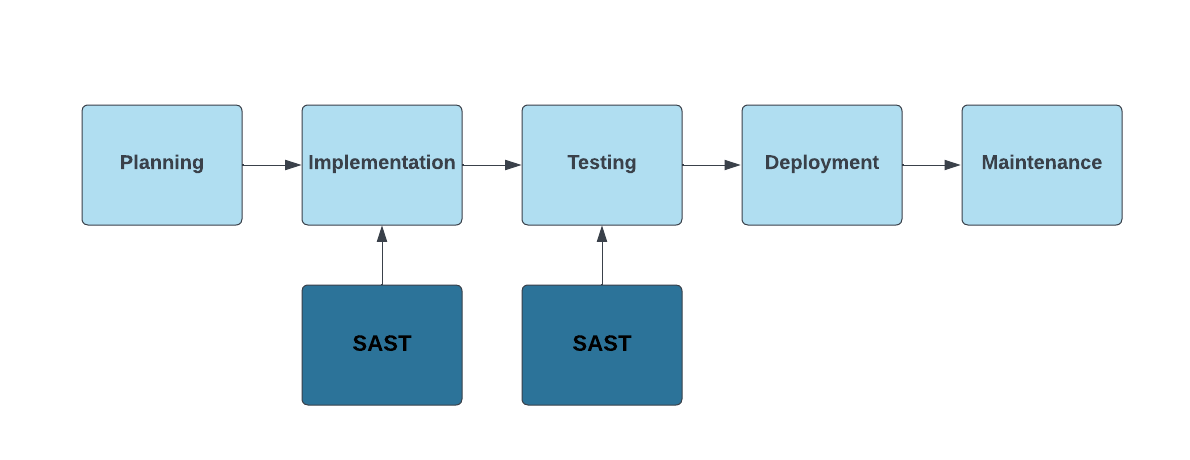
\includegraphics[width=0.8\columnwidth]{Images/sast.png}
    \caption{SAST tools are introduced early in the SDLC and can help identify vulnerabilities during the implementation and testing phases}
    \label{fig: Where SAST can be performed in SDLC}
\end{figure}

\subsection{DAST}
\acrlong{dast} (\acrshort{dast}) uses a black box testing technique that evaluates the security of an application by performing security assessments of a running instance of the application \cite{dast}. Unlike \acrshort{sast}, which analyzes the source code of an application, \acrshort{dast} evaluates the application as its being used. The evaluation includes the interaction of different components and the runtime environment. 
\\~\\
\acrshort{dast} simulates real-world attacks, which is done by sending malicious requests and inputs to the application it is testing and then monitoring the responses. In the end, the tool generates a report that includes the identified vulnerabilities, including a more in-depth description and remediation on how to fix the issue. 
\\~\\
An advantage with \acrshort{dast} is that it can identify security issues that are not detectable through \acrshort{sast}. These security issues can, for example, be interactions between different components. Another advantage is that with \acrshort{dast}, it can identify different vulnerabilities that get triggered, for example, when the application is under heavy load or when specific inputs are received.
\\~\\
However, there are some limitations with \acrshort{dast} as well, one being that it can only detect vulnerabilities present in the deployed version of the application and cannot give an in-depth description of vulnerabilities that lie in the source code. Additionally, \acrshort{dast} can generate several false positives, increasing the testing time and effort required to analyze and verify the results. 
\\~\\
In Figure \ref{fig: Where DAST can be performed in SDLC}, \acrshort{dast} is suggested to perform in the testing and maintenance phase since the scan is done on a running application and is, therefore, past the implementation stage. The test should be done before deployment to prevent a vulnerable application from going public. Scans should also be done after it is deployed, in the maintenance phase, since vulnerabilities may occur after deployment and must be identified to prevent potential problems. 

\vspace{2mm}
\begin{figure}[H]
    \centering
    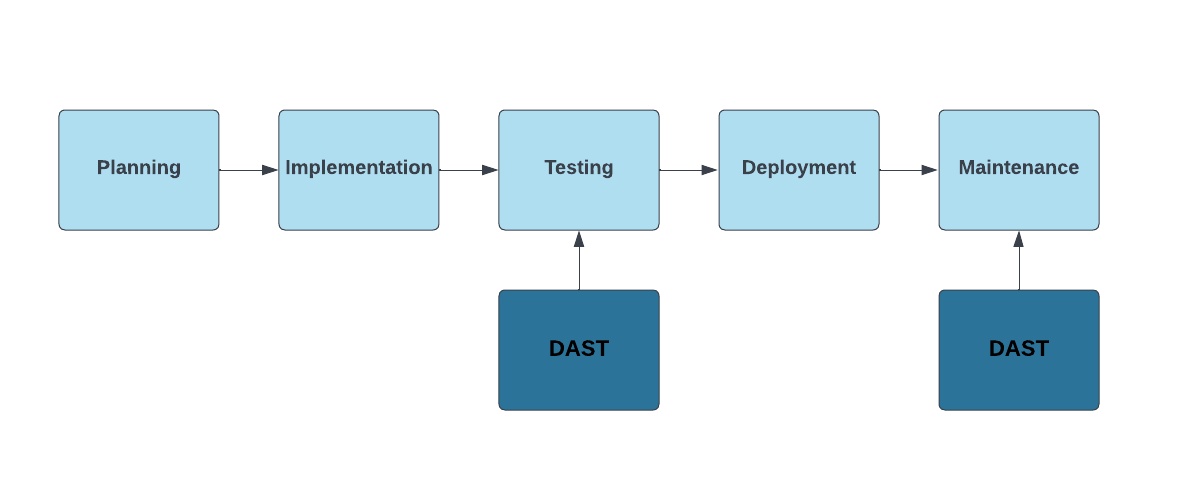
\includegraphics[width=0.8\columnwidth]{Images/dast.png}
    \caption{Where DAST can be performed in SDLC} 
    \label{fig: Where DAST can be performed in SDLC}
\end{figure}

\subsection{SCA}
\acrlong{sca} (\acrshort{sca}) is a type of grey box testing that analyzes the dependencies of a software application to identify and manage potential security risks \cite{sca}. The main objective of the \acrshort{sca} is to identify third-party components that may contain security vulnerabilities. 
\\~\\
\acrshort{sca} scans the application's code to identify all of its \gls{dependency}, including the different versions of the components used. It then cross-references these \gls{dependency} to different databases with known vulnerabilities and generates a report containing any potential risk. Compared to the other tests, the report also includes an in-depth description of the vulnerability and a recommendation to update the components to newer versions or replace these. 
\\~\\
An advantage with \acrshort{sca} is that it can quickly identify risks that may be introduced from third-party components. It is relatively common that modern applications rely on many different dependencies, making \acrshort{sca} useful. It can provide a comprehensive view of the security risks associated with an application and help developers make informed decisions about the security of the developed applications. 
\\~\\
However, \acrshort{sca} may give some false positives that can occur because one has an extensive library in the code. In addition, it can trigger because of a dependency that is never used and is, therefore, impossible to exploit.
\\~\\
\acrshort{sca} scans are done at an early stage in modern software development \cite{scaplasment}. Shown in Figure \ref{fig: DevSecOps Life Cycle} it is performed in the build stage. Therefore, Figure \ref{fig: Where SCA can be performed in SDLC} suggests \acrshort{sca} scans to be performed in the implementation phase. The scan is also suggested in the testing and maintenance phases. The testing phase is an alternative or an addition to the implementation phase. The maintenance phase should include checks, as dependencies may become vulnerable after deployment.

\vspace{2mm}
\begin{figure}[H]
    \centering
    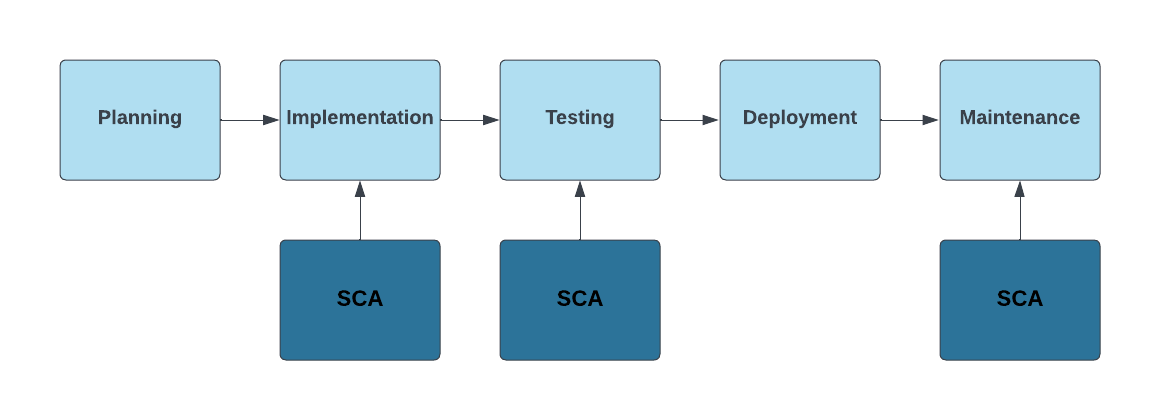
\includegraphics[width=0.8\columnwidth]{Images/sca.png}
    \caption{Where SCA can be performed in SDLC} 
    \label{fig: Where SCA can be performed in SDLC}
\end{figure}

\newpage
\subsection{Comparison of SAST, DAST, and SCA}
Upon reviewing the different security application tests, similarities between \acrshort{sast}, \acrshort{dast}, and \acrshort{sca} were discovered. Table \ref{fig: Comparison of SCA, DAST, and SASt} below shows some commonalities and differences, which indicates that a combination of the different testing mechanisms can enhance the testing process of the application. 

\vspace{2mm}
\begin{figure}[H]
    \centering
    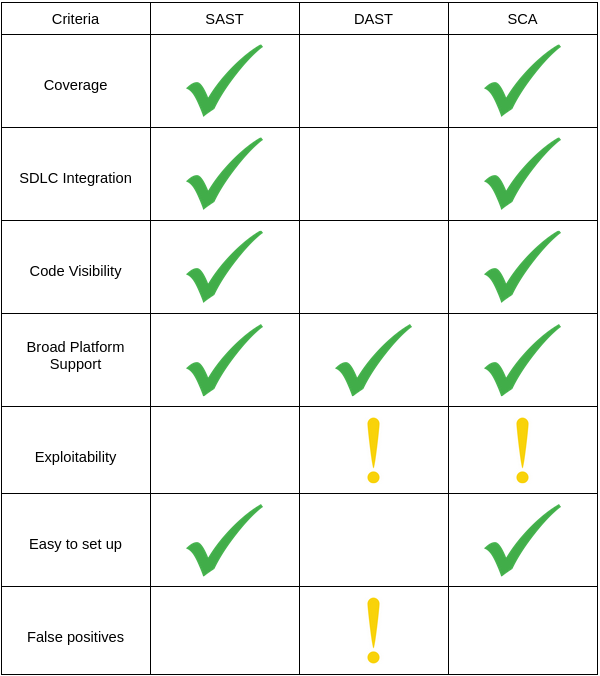
\includegraphics[width=0.8\columnwidth]{Images/application-security-testing.png}\\
    \textbf{Note:} The distinction between the exclamation marks and the checkmarks lies in the meaning of them. The exclamation marks indicate that the criteria are considered negative, while the checkmarks signify that the criteria are positive.
    \caption{Comparison of SCA, DAST, and SAST}Adapted from: \cite{Comparison}
    \label{fig: Comparison of SCA, DAST, and SASt}
\end{figure}

\section{The significance of software security testing}
Security testing plays a critical role in the \acrlong{sdlc}, as it is employed to identify potential security vulnerabilities in the system and prevent real-world attacks \cite{whysectest}. It is a process where the system's security is evaluated, and its possible security weaknesses and vulnerability risks are identified. 
\\~\\
According to IBM's report, in 2022, the cost of a data breach was estimated to be USD 4.35 million \cite{databreach}. Investing in cybersecurity measures can save money for a company in the event of a cyber attack. The report states that companies that have implemented zero trust security measures saved about USD 1 million in breach costs on average compared to those that have not. To repair a vulnerability in the design phase costs an average of USD 500 \cite{fixvulnerability}. Starting software testing early in the SDLC reduces costs and saves time. As mentioned in section \ref{Functional Testing vs Security Testing}, various types of testing should be executed on an application, including testing of both the written code and the libraries that are integrated and being used.

\section{OWASP Top 10}
\acrlong{owasp} (\acrshort{owasp}) serves as a standard reference document for web application security and for developers to raise their knowledge of potential security threats. The document contains a prioritized and exemplified list with recommendations for fixing ten critical security flaws commonly seen in web applications. The function of this document is to educate readers on the most common security risks that may occur. Developers and security professionals may use this knowledge and implement it into their security policies, reducing the frequency of these dangers in their applications. 




\section{Vulnerability risk rating}
Discovered vulnerabilities can be rated by standardized systems like CVSS, CVE, CWE, and OWASP Risk Rating Methodology. These databases are frequently used in application security testing, particularly in SCA scans, to uncover code patterns that may indicate a common vulnerability within the code. While they may also be utilized in DAST and SAST scans, they are most commonly used in SCA scans. 

\subsection{Common Vulnerability Scoring System (CVSS)}
\acrlong{cvss}, known as \acrshort{cvss}, is \textit{"a Security Content Automation Protocol (SCAP) specification for communicating the characteristics of vulnerabilities and measuring their relative severity"}\cite{nistCVSS}. The system is used to give vulnerabilities a numeric score based on their severity. The scores can be translated into low, medium, high, and critical to assist organizations in evaluating and ranking their vulnerabilities. CVSS is currently at version 3.1. \cite{CVSS}

\begin{figure}[H]
    \centering
    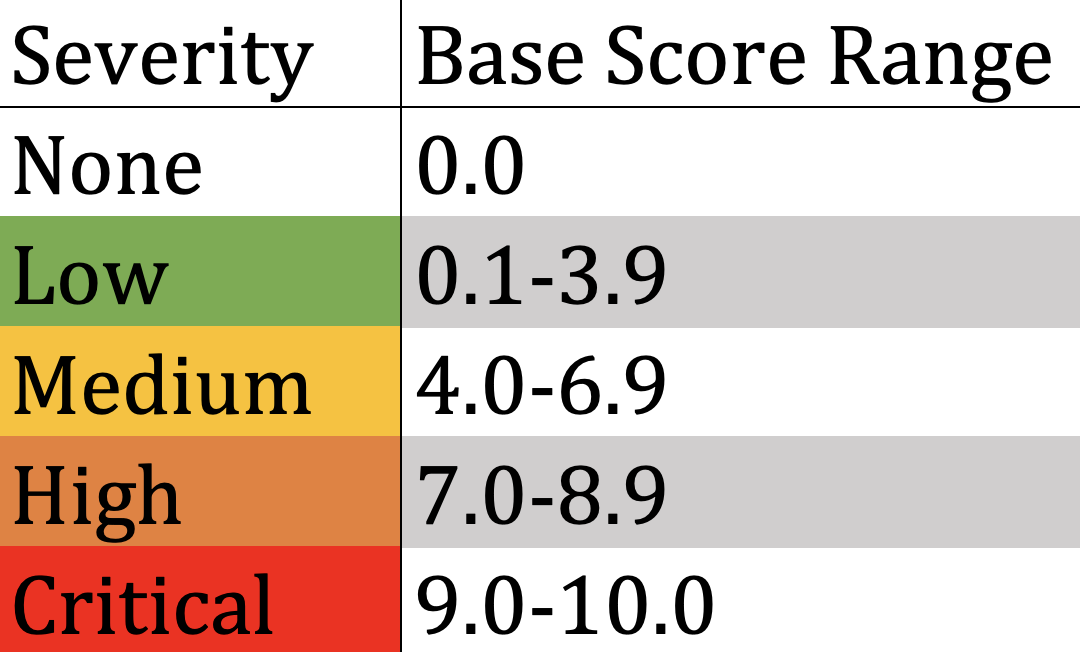
\includegraphics[scale=0.3]{Images/CVSS.png}
    \caption{CVSS v3 Ratings} Adapted from:\cite{cvssrating}
    \label{fig:CVSS v3 Ratings}
\end{figure}

\subsection{Common Vulnerabilities and Exposures (CVE)}
\label{Common Vulnerabilities and Exposures}
\acrlong{cve}\footnote{Available at \url{https://www.cve.org/}}, known as \acrshort{cve}, is, according to their website,\textit{"a list of records each containing an identification number, a description, and at least one public reference for publicly known cybersecurity vulnerabilities"}\cite{CVE}. The CVE program aims to determine, describe, and categorize cybersecurity vulnerabilities made public. All discovered vulnerabilities will be put into records and sent to \acrlong{nvd} (\acrshort{nvd})\footnote{Available at: https://nvd.nist.gov}, which is a list of vulnerabilities maintained by the United States government.

\subsection{Common Weakness Enumeration (CWE)}
\label{cwe}
\acrlong{cwe}\footnote{Available at \url{https://cwe.mitre.org/}}, know as \acrshort{cwe}, is \textit{"a community-developed list of common software and hardware weakness types that have security ramifications"}\cite{CWE}. It was established to serve as a consistent benchmark for security solutions that address vulnerabilities and as a baseline for identifying, mitigating, and preventing weaknesses. CWE's goal is to provide instructions for those who have control over and maintain source code to stop the vulnerabilities at the source. 

\subsection{OWASP Risk Rating Methodology}
\acrshort{owasp} Risk Rating Methodology contains a formula that calculates a risk score for each vulnerability based on likelihood and impact \cite{owasprisk}. Multiple factors make up both likelihood and impact. 
\\~\\
Factors composing the estimation of likelihood are separated into different groups related to the threat actor and the vulnerability. The set of factors related to the threat actor is skill level, motive, opportunity, and size. The factors related to the vulnerability are the ease of discovery, ease of exploit, awareness, and intrusion detection. Each factor will have different options and receive a likelihood rating from 0-9. 
\\~\\
Factors composing the estimation of impact are divided into technical and business impacts. The technical impact is broken down into confidentiality, integrity, availability, and accountability. Further, the business impact is divided into financial damage, reputation damage, non-compliance, and privacy violation. All of the factors will receive an impact rating from 0-9. 
\\~\\
Combining the likelihood and impact factors estimates produces an overall severity level of the risk, which can be classified as low, medium, or high (as shown in figure \ref{fig: Impact levels}) to determine its severity. These levels can be further combined to determine the final severity of the risk, as illustrated in figure \ref{fig: OWASP Severity Scale}.


\vspace{2mm}
\begin{figure}[H]
    \centering
    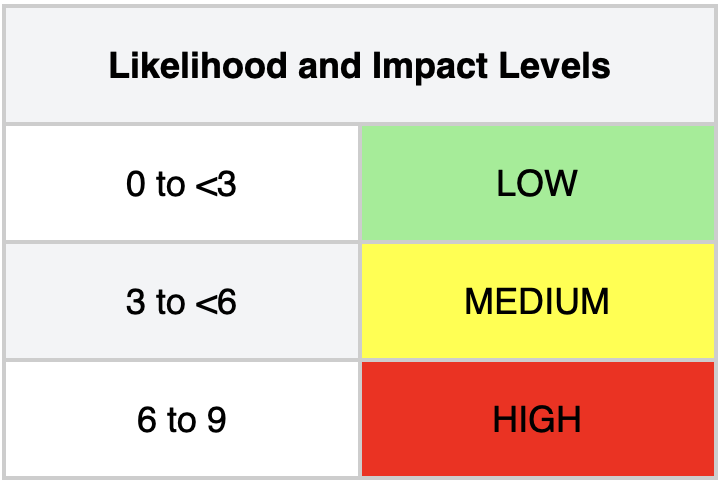
\includegraphics[scale=0.5]{Images/OWASP-likelihood.png}
    \caption{The likelihood and impact levels}
    \label{fig: Impact levels}
\end{figure}

\vspace{2mm}
\begin{figure}[H]
    \centering
    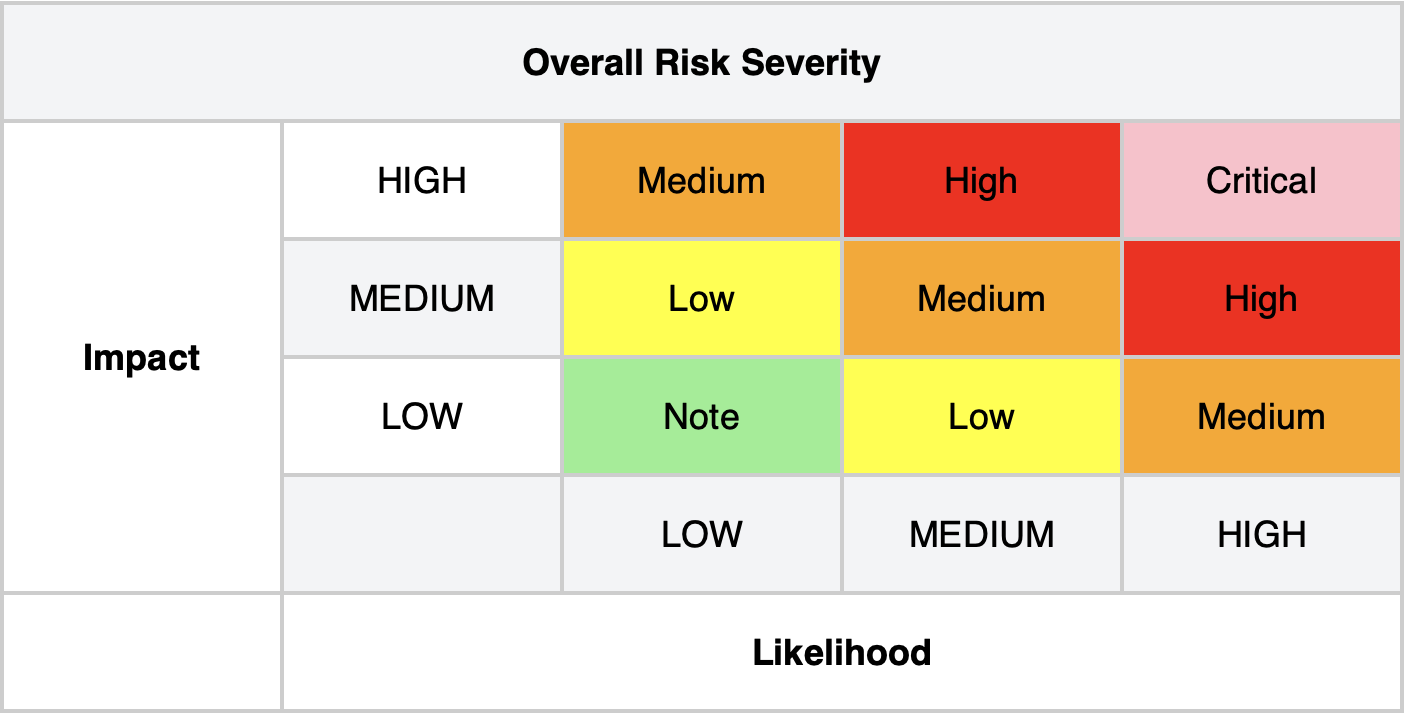
\includegraphics[scale=0.4]{Images/OWASP-severity.png}
    \caption{Severity level based on impact and likelihood}
    \label{fig: OWASP Severity Scale}
\end{figure}

\section{Amazon Web Services}
\acrlong{aws}\footnote{Available at \url{https://aws.amazon.com/}}, known as \acrshort{aws}, is a cloud computing platform offered by Amazon. It provides a variety of services ranging from \acrlong{iaas} (\acrshort{iaas}) to \acrlong{paas} (\acrshort{paas}), enabling customers to operate their applications and store their data in the cloud. With their pay-as-you-go cloud computing model, customers can scale their resources up and down without investing in physical infrastructure.\cite{aws}  

\section{GitHub}
GitHub\footnote{Available at \url{https://github.com/}} is a web-based software development platform where developers can collaborate and store open and closed-source projects. The developers can manage their projects in repositories and track bugs and issues. It offers collaboration tools, including pull requests, code reviews, and project management functionalities. Git is a version control system utilized to manage and monitor file versioning. GitHub employs this technology as the basis for its service. This allows developers to work on code simultaneously, track changes, and merge contributions from multiple contributors.\cite{github}
